\let\negmedspace\undefined
\let\negthickspace\undefined
\documentclass[journal]{IEEEtran}
\usepackage[a5paper, margin=10mm, onecolumn]{geometry}
\usepackage{lmodern} % Ensure lmodern is loaded for pdflatex
\usepackage{tfrupee} % Include tfrupee package

\setlength{\headheight}{1cm} % Set the height of the header box
\setlength{\headsep}{0mm}     % Set the distance between the header box and the top of the text

\usepackage{gvv-book}
\usepackage{gvv}
\usepackage{cite}
\usepackage{amsmath,amssymb,amsfonts,amsthm}
\usepackage{algorithmic}
\usepackage{graphicx}
\usepackage{textcomp}
\usepackage{xcolor}
\usepackage{txfonts}
\usepackage{listings}
\usepackage{enumitem}
\usepackage{mathtools}
\usepackage{gensymb}
\usepackage{comment}
\usepackage[breaklinks=true]{hyperref}
\usepackage{tkz-euclide} 
\usepackage{listings}
\def\inputGnumericTable{}                                 
\usepackage[latin1]{inputenc}                                
\usepackage{color}                                            
\usepackage{array}                                            
\usepackage{longtable}                                       
\usepackage{calc}                                             
\usepackage{multirow}                                         
\usepackage{hhline}                                           
\usepackage{ifthen}                                           
\usepackage{lscape}

\begin{document}

\bibliographystyle{IEEEtran}
\vspace{3cm}

\title{9.1.3}
\author{EE24BTECH11047 - Niketh Prakash Achanta}
% \maketitle
% \newpage
% \bigskip
{\let\newpage\relax\maketitle}

\renewcommand{\thefigure}{\theenumi}
\renewcommand{\thetable}{\theenumi}
\setlength{\intextsep}{10pt} % Space between text and floats

\textbf{Question:}
\newline
Solve the differential equation:
\begin{align}
	x y^{\prime\prime} + 2y^{\prime} - x y + x^2 - 2 = 0
\end{align}

\textbf{Solution:}

\textbf{Theoretical solution:}
\newline
The given differential equation is a second-order nonlinear ordinary differential equation and cannot be theoretically solved using known methods.
\newline
\textbf{Computational Solution:} Euler's method
\newline
By the first principle of derivative,
\begin{align}
    y^{\prime}\brak{x} &= \lim_{h\to0} \frac{y\brak{x + h} - y\brak{x}}{h}\\
    y\brak{x + h} &= y\brak{x} + h\brak{y^{\prime}\brak{x}}, h\to0
\end{align}

For a $m^{\text{th}}$ order differential equation,
\newline

Let 
\begin{align}
    y_1 = y \text{ , } y_2 = y^{\prime} \text{ , } y_3 = y^{\prime\prime} \text{ , } \dots \text{ , } y_m = y^{m - 1}
\end{align}
then we obtain the system

\begin{align}
    \myvec{y_1^{\prime}\\y_2^{\prime}\\\vdots\\y_{m - 1}^{\prime}\\y_m^{\prime}} = \myvec{y_2\\y_3\\\vdots\\y_m\\f\brak{x, y_1, y_2,\dots,y_m}}
\end{align}
Here, $f$ is described by the given differential equation. The initial conditions $y_1\brak{x_0} = K_1$, $y_2\brak{x_0} = K_2$, $\dots$, $y_m\brak{x_0} = K_m$.

Representing the system in Euler's form \brak{\text{using first principle of derivative}},
\begin{align}
    \myvec{y_1\brak{x + h}\\y_2\brak{x + h}\\\vdots\\y_m\brak{x + h}} &= \myvec{y_1\brak{x} + hy_2\brak{x}\\y_2\brak{x} + hy_3\brak{x}\\\vdots\\y_m\brak{x} + hf\brak{x, y_1, y_2 \dots y_m}}\\
    \myvec{y_1\brak{x+h} \\ \vdots \\ y_{m-1}\brak{x+h} \\ y_m\brak{x+h}} &=\myvec{y_1\brak{x} \\ \vdots \\ y_{m-1}\brak{x} \\ y_m\brak{x}} + h\myvec{y_2\brak{x} \\ \vdots \\ y_m\brak{x} \\f\brak{x, y_1, y_2, \dots, y_m} }\\
    \vec{y}\brak{x+h} &= \vec{y}\brak{x} + h\myvec{0 & 1 & 0 & 0 & \dots & 0 & 0\\ 0 & 0 & 1 & 0 & \dots & 0 & 0\\0 & 0 & 0 & 1 & \dots & 0 & 0\\\vdots & \vdots & \vdots & \vdots& \ddots & \vdots & \vdots\\ 0 & 0 & 0 & 0 & \dots & 0 & 1\\0 & 0 & 0 & 0 & \dots & 0 &\frac{f\brak{x, y_1, y_2, \dots, y_m}}{y_m}}\vec{y}\brak{x}\\
    \vec{y}\brak{x+h} &= \myvec{1 & h & 0 & 0 & \dots & 0 & 0\\ 0 & 1 & h & 0 & \dots & 0 & 0\\0 & 0 & 1 & h & \dots & 0 & 0\\\vdots & \vdots & \vdots & \vdots& \ddots & \vdots & \vdots\\ 0 & 0 & 0 & 0 & \dots & 1 & h\\0 & 0 & 0 & 0 & \dots & 0 & 1+\frac{f\brak{x, y_1, y_2, \dots, y_m}}{y_m}}\vec{y}\brak{x}
\end{align}

Generalizing the system into an iterative format for plotting $y\brak{x}$,
\begin{align}
    \myvec{y_{1, n + 1}\\y_{2, n + 1}\\\vdots\\y_{m, n + 1}} &= \myvec{y_{1, n}\\y_{2, n}\\\vdots\\y_{m, n}} + h\myvec{y_{2, n}\\y_{3, n}\\\vdots\\f\brak{x_n, y_{1, n}, y_{2, n}, \dots, y_{m, n}}}\\
    \vec{y_{n + 1}} &= \vec{y_{n}} + h\myvec{0 & 1 & 0 & 0 & \dots & 0 & 0\\ 0 & 0 & 1 & 0 & \dots & 0 & 0\\0 & 0 & 0 & 1 & \dots & 0 & 0\\\vdots & \vdots & \vdots & \vdots & \ddots & \vdots & \vdots\\ 0 & 0 & 0 & 0 & \dots & 0 & 1\\0 & 0 & 0 & 0 & \dots & 0 & \frac{f\brak{x_n, y_{1, n}, y_{2, n}, \dots, y_{m, n}}}{y_{m, n}}}\vec{y_n} \text{, where } \vec{y_n} = \myvec{y_{1, n}\brak{x_n}\\y_{2, n}\brak{x_n}\\\vdots\\y_{m, n}\brak{x_n}}\\
    \vec{y_{n + 1}} &= \myvec{1 & h & 0 & 0 & \dots & 0 & 0\\ 0 & 1 & h & 0 & \dots & 0 & 0\\0 & 0 & 1 & h & \dots & 0 & 0\\\vdots & \vdots & \vdots & \vdots& \ddots & \vdots & \vdots\\ 0 & 0 & 0 & 0 & \dots & 1 & h\\0 & 0 & 0 & 0 & \dots & 0 & 1+\frac{f\brak{x_n, y_{1, n}, y_{2, n}, \dots, y_{m, n}}}{y_{m, n}}}\vec{y_n}\\
    x_{n + 1} &= x_{n} + h
\end{align}
Here, the vector $\vec{y_n}$ is not to be confused with $y_k$ which is the $\brak{k - 1}^{\text{th}}$ derivative of $y\brak{x}$.
\newline
The given differential equation can be represented as,
\begin{align}
    \brak{y^{\prime}}^4 + 3yy^{\prime\prime} = 0\\
    y^{\prime\prime} = -\frac{\brak{y^{\prime}}^4}{3y}
\end{align}
Here $m = 2$, thus,
\begin{align}
    y_3 &= y^{\prime\prime} = -\frac{\brak{y^{\prime}}^4}{3y} = -\frac{\brak{{y_2}^4}}{3y_1}\\
    \myvec{y_1^{\prime}\\y_2^{\prime}} &= \myvec{y_2\\-\frac{\brak{y^{\prime}}^4}{3y}}\\
    \myvec{y_{1, n + 1}\\y_{2, n + 1}} &= \myvec{y_{1, n}\\y_{2, n}} + h\myvec{y_{2, n}\\-\frac{\brak{y_{2, n}}^4}{3y_{1, n}}}\\
    \vec{y_{n + 1}} = \myvec{1 & h\\0 & 1 -\frac{\brak{y_{2, n}}^3}{3y_{1, n}}} \vec{y_n}
\end{align}

Iteratively plotting the above system taking initial conditions as 
\begin{align}
    x_0 = 0 \text{ , } y_{1, 0} = 0.01 \text{ , } y_{2, 0} = 1
\end{align}
we get the following plot.

\begin{figure}[h!]
   \centering
   \includegraphics[width=0.7\columnwidth]{figs/graph.png}
   \caption{Computational solution for $\brak{y^{\prime}}^4 + 3yy^{\prime\prime} = 0$}
   \label{label}
\end{figure}
\begin{figure}[!ht]
    \centering
    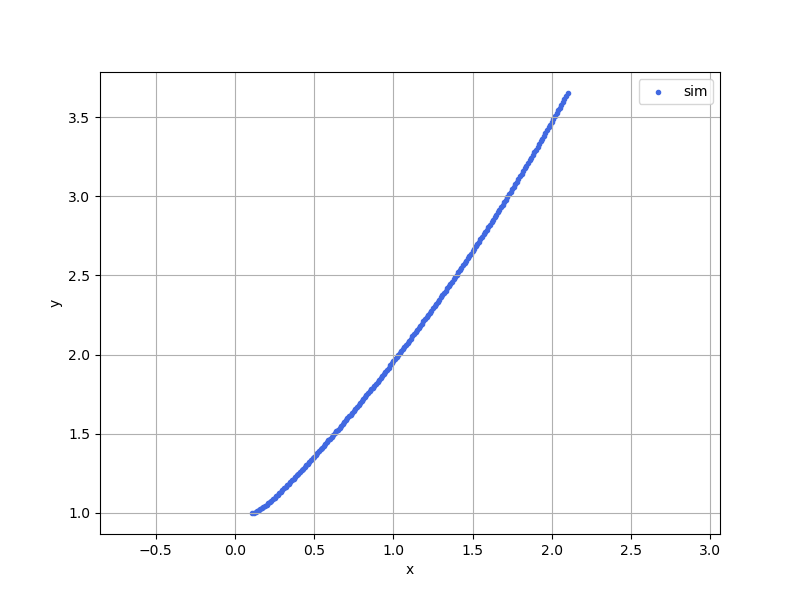
\includegraphics[width=\columnwidth]{/home/niketh/EE1003/Assignment-1/figs/fig1.png}
    \caption{}
\end{figure}
\end{document}
